\documentclass[handout]{beamer}
\usepackage{amsfonts}
\usepackage{amsmath}

\usetheme{Madrid}

\title[ALARI Statistics Course]{ALARI Statistics Course}
\subtitle{Part II}
\author[Claudio Ortelli]{Claudio Ortelli}
\institute[USI]{Universit\`{a} della Svizzera italiana}
\date[29/2010]{April 2011}

\begin{document}
\maketitle
\section{Function of random variables}
\begin{frame}{Function of random variables}
\begin{itemize}
  \item Let $X$ be a continous random variable with distribution function
  $F_X$, $\Psi$ a function and \[ Y = \Psi(X) .\]
  \item Under regularity conditions on $\Psi$, $Y$ is a random variable!
  \item Continuity or stepwise continuity of $\Psi$ are sufficient conditions
  for $Y$ to be a random variable
  \item 
\end{itemize}
\end{frame}

 
\section{Simulation of random variables}
\begin{frame}{Simulation of random variables}{Motivation}
\begin{itemize}
 \item We are interested in simulating a model of a real system (network, electronic device, ...).
 \item The output $Y$ of the model depends on a stochastic input, i.e. a random variable $X$ with known distribution 
function $F_X$: 
\[ Y = g(X). \]
\end{itemize}
\begin{center}
 \includegraphics[width=157pt,keepaspectratio=true]{./sistemaComplesso.png}
 % sistemaComplesso.png: 314x158 pixel, 72dpi, 11.08x5.57 cm, bb=0 0 314 158
\end{center}
\end{frame}


\begin{frame}{Simulation of random variables}{}
\begin{itemize}
 \item The model is too complex in order to analytically derive the probabilistic properties of the output, i.e. $F_Y$.
 \item Idea: simulate a possible outcome $x$ of the input $X$ and evaluate the corresponding outcome $y=g(x)$ of the output. Repeat the experiment 
$N$ times and analyse the results.
 \item The simulated values of the input must be drawn from the distribution of $X$.
 \item Question: how is it possible to simulate independent realizations from a given distribution $F_X$?
 \item Answer: different methods available. The simplest of them requires simulating from the uniform distribution on the open interval (0,1), 
  i.e. $U(0,1)$. In Matlab use the function ``rand''.
\end{itemize}
\end{frame}

\begin{frame}{Simulation of random variables}{Inverse Transform Method}
If the distribution function $F_X$ is continuous and strictly increasing then $F_X^{-1}:\ (0,1)\rightarrow \mathbb{R}$ exists. \\
\begin{center}
Example: Chi-Squared Distribution with 5 degrees of freedom
 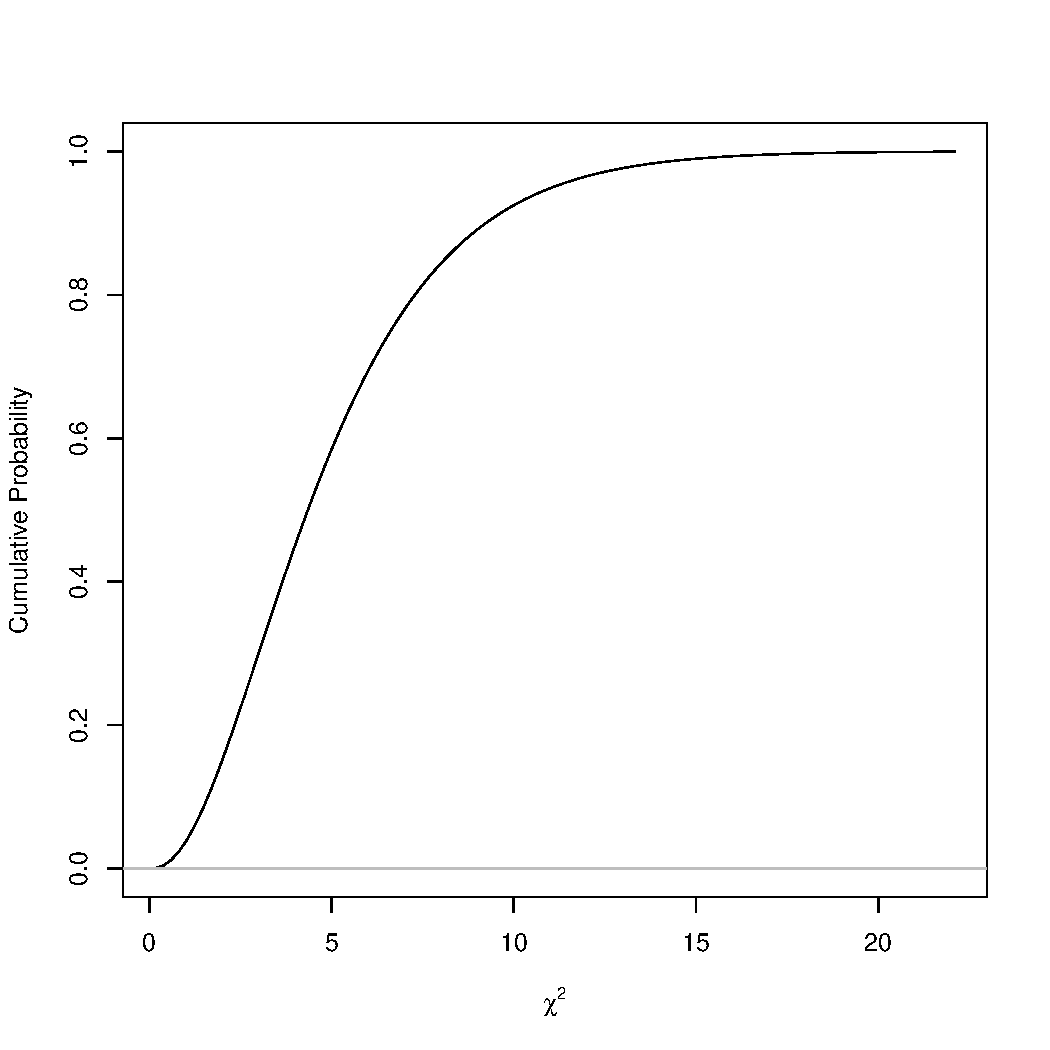
\includegraphics[width=5.8cm,keepaspectratio=true]{./distChi2.pdf}
 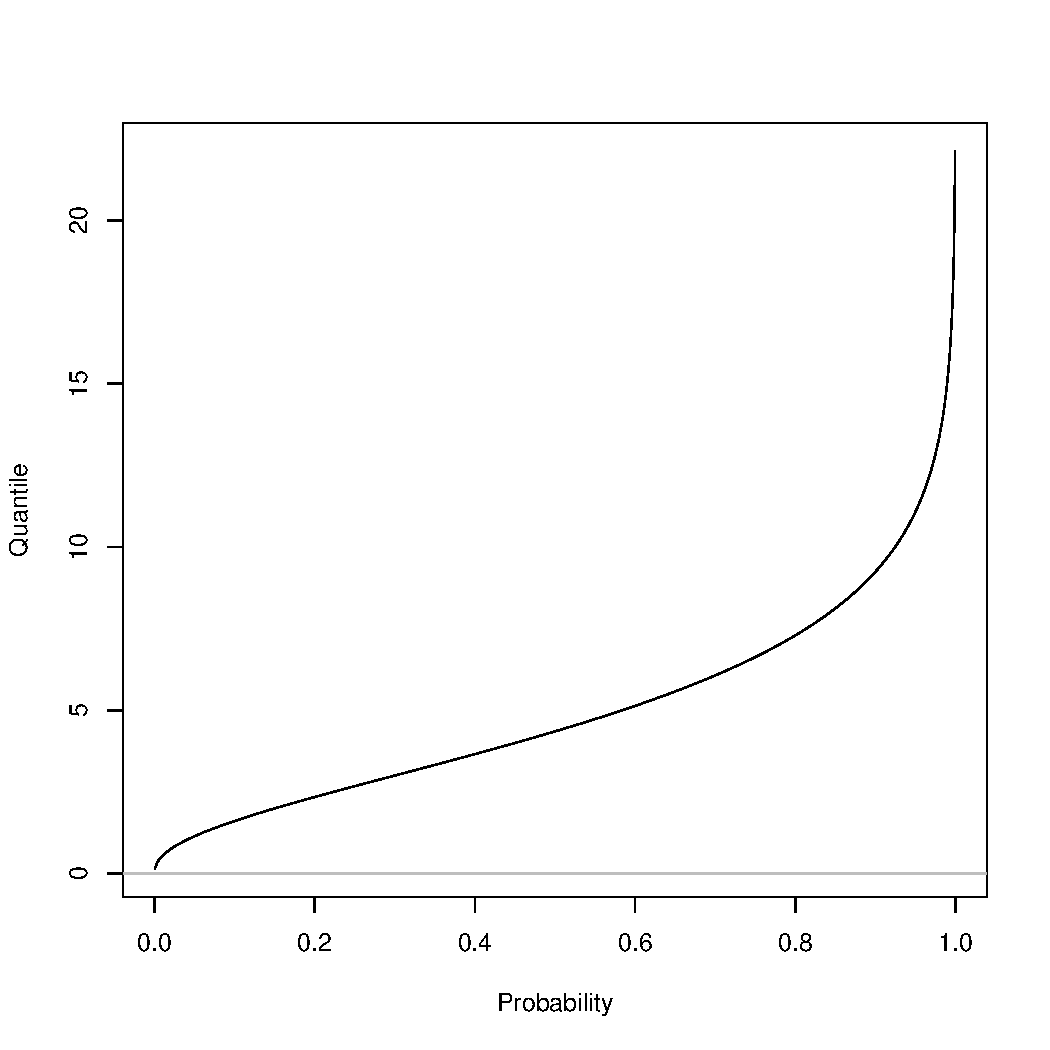
\includegraphics[width=5.8cm,keepaspectratio=true]{./quantileChi2.pdf}
\end{center}
\end{frame}

\begin{frame}{Simulation of random variables}
For a general distribution function not necessarily strictly increasing define 
\[F_X^{-1}(p) = \inf \{x : p \leq F_X(x) \}  \ \ 0 < p < 1.\]
It then follows that
$F_X^{-1}(p) \leq x   \Longleftrightarrow p \leq F_X(x).$
\vspace{0.2cm}
\begin{center}
Example: Binomial distribution $Bin(n=3,p=0.3)$ 
\end{center}
\vspace{-0.7cm}
\begin{center}
 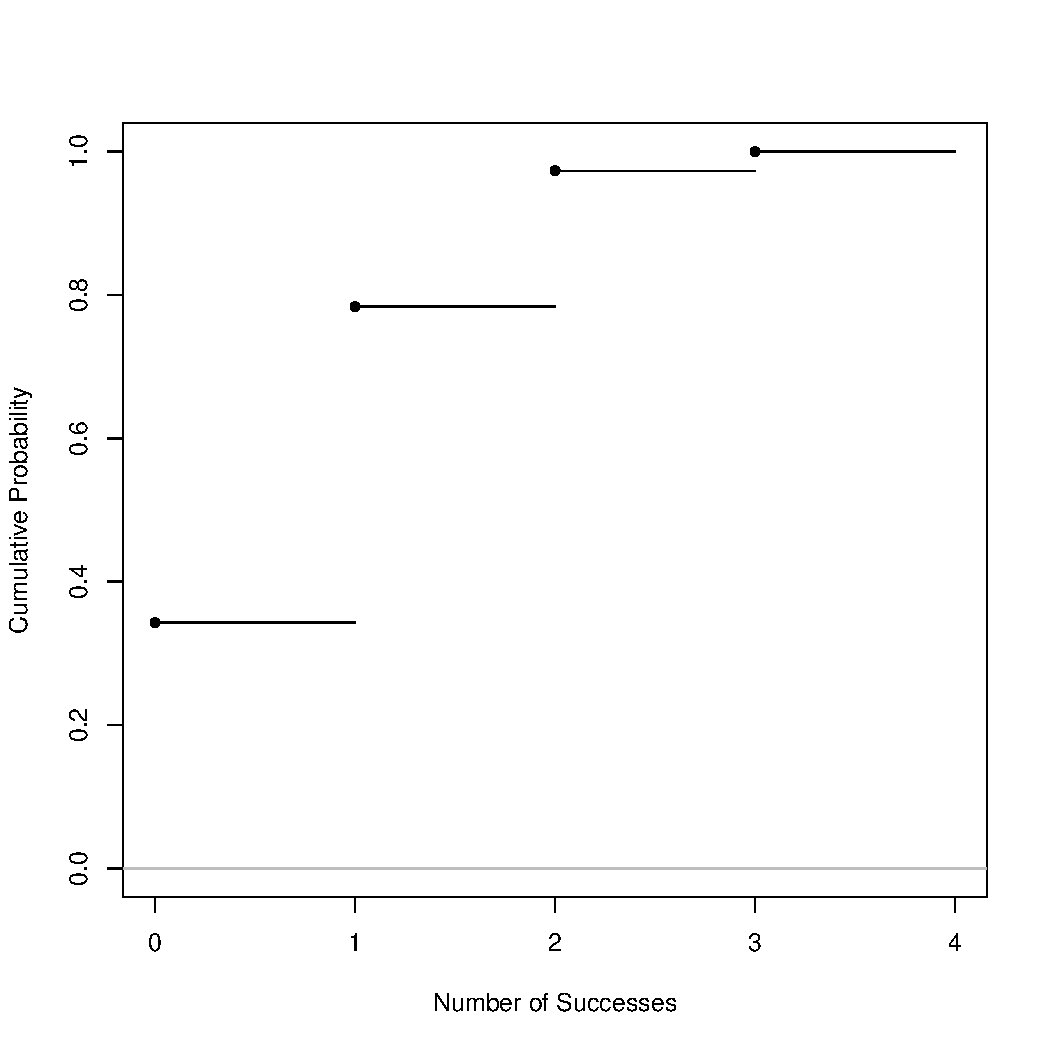
\includegraphics[width=5.8cm,keepaspectratio=true]{./distBinomiale.pdf}
 \includegraphics[width=5.8cm,keepaspectratio=true]{./quantileBinomiale.pdf}
\end{center}
\end{frame}

\begin{frame}{Simulation of random variables}{Inverse Transform Method}
\begin{theorem}[Inverse Transform Method]
Let $U$ a continuous Unif(0,1) distributed random variable. The random variable $Y=F_X^{-1}(U)$ has distribution 
function $F_X$.
\end{theorem}
\begin{proof}
By definition 
\[ F_Y(c) := P(Y \leq c) = P(F_X^{-1}(U)\leq c).
\]
But the last equality is equivalent to (see previous slide) 
\[
P(U\leq F_X(c)) = F_X(c).
\]
\end{proof}
\end{frame}


\begin{frame}{Simulation of random variables}{Inverse Transform Method}
From the previous theorem we derive the following \emph{two steps} simulation algorithm
\begin{itemize}
  \item<1->Simulate a realization $u$ from a Unif(0,1) random variable $U$.
  \item<2-> Compute $x = F_X^{-1}(u)$.
\end{itemize}
\vspace{0.8cm}
Example: Simulation of $Y \sim Exp(\lambda)$
\begin{itemize}
 \item The distribution function is $F_Y(x)=1-\exp(-\lambda x)$
 \item Compute $F^{-1}_Y(p)=-\frac{1}{\lambda}\ln(1-p)$
 \item Sample a random draw $u$ from $U \sim$ Unif(0,1)
 \item Set $y = -\frac{1}{\lambda}\ln(1-u)$
\end{itemize}
\end{frame}


\begin{frame}{Simulation of random variables}{Inverse Transform Method}
\vspace{-4cm}
Remark: if $U \sim$ Unif(0,1) then $1-U$ is also Unif(0,1). Therefore we can 
also write $Y = -\frac{1}{\lambda}\ln(U)$.
\end{frame}

\begin{frame}{Simulation of random variables}{Inverse Transform method}
For a descrete random variable $Y$ with probability mass function $P(Y=x_i)=p_i$, $i=1, ...,m$ 
consider the following algorithm:
\begin{enumerate}
 \item Generate a Unif(0,1) random variable $U$
 \item Compute $Y$ as follows
\[
 Y = x_j \textnormal{\hspace{0.5cm} if \hspace{0.1cm}} \sum_{i=1}^{j-1} p_i < U \leq  \sum_{i=1}^{j} p_i.
\]
i.e. $Y = x_j$ if $F_Y(x_{j-1})< U \leq F_Y(x_j)$.
\end{enumerate}
\end{frame}


\begin{frame}{Simulation of random variables}{Inverse Transform method}
Example: let $Y$ have the following mass function 
\begin{center}
\begin{tabular}{|c|c|c|c|}
\hline
$p_1$ & $p_2$ & $p_3$ & $p_4$\\ \hline
0.1 & 0.2 & 0.4 & 0.3 \\
\hline
\end{tabular}
\end{center}
The simulation algorithm is the following:
\begin{enumerate}
 \item If $u \leq p_1 = 0.1$ then $y=x_1$. Stop.
 \item if $u \leq p_1 + p_2 = 0.3$ then $y=x_2$. Stop.
 \item if $u \leq p_1 + p_2 + p_3 = 0.7$ then $y=x_3$. Stop.
 \item $y=x_4$. Stop.
\end{enumerate}
This algorithm is correct but inefficient. In fact, probabilities of one, two, ...
comparisons are equal to the probabilities of $x_1$, $x_2$, ..., respectively.
The expected number of comparisons is \[ p_1 + 2 p_2 + 3 p_3 + 4 p_4 = 2.9 .\]
\end{frame}

\begin{frame}{Simulation of random variables}{Inverse Transform method}
We can improve efficiency by sorting the values of $x_i$ by decreasing order 
of probabilities $p_i$'s: $x_3$, $x_4$, $x_2$ and $x_1$.
\begin{enumerate}
 \item If $u \leq p_3 = 0.4$ then $y=x_3$. Stop.
 \item if $u \leq p_3 + p_4 = 0.7$ then $y=x_4$. Stop.
 \item if $u \leq p_3 + p_4 + p_2 = 0.9$ then $y=x_2$. Stop.
 \item $y=x_1$. Stop.
\end{enumerate}
\vspace{1cm}
The expected number of comparisons is now equal to 
\[ p_3 + 2 p_4 + 3 p_2 + 4 p_1 = 2 .\]
\end{frame}

\begin{frame}{Simulation of random variables}{Exercises}
The Laplace distribution is a continuous distribution with density function
\[f(x;\mu,b)=\left\{\begin{array}{ll}
\frac{1}{2b}\exp(- \frac{\mu - x}{b}) & \textnormal{if } x < \mu\\
\frac{1}{2b}\exp(- \frac{x - \mu}{b}) & \textnormal{if } x \geq \mu
\end{array} \right.
\]
where $\mu$ is the mean and $b$ a scale parameter.
\begin{enumerate}
\item Plot the density, distribution and quantile functions of the Laplace distribution with parameter 
$\mu=1$ and $b=0.5$.
\item Using the previous values of $\mu$ and $b$ simulate $N=1000$ independent realizations of a Laplace distributed random variable $Y$.
\item Plot the histogram of the simulated random variables and compare it with the density function of $Y$.
\item Plot the empiric distribution function of the simulated sample and compare it with the distribution function of $Y$.
\end{enumerate}
\end{frame}

\begin{frame}{Simulation of random variables}{Transform methods}
The theorem on \emph{Distributions of functions of continuous random variables} allows us to
generate random variables by means of ad hoc transformations of Unif(0,1) random variables. The following theorem generalizes
the previous theorem to the multivariate case.
\begin{Theorem}
Assume that $X=(X_1,X_2)$ is a random vector with joint density function $f_X(x_1,x_2)$ and $g: \mathbb{R}^2 \rightarrow \mathbb{R}^2$ a one-to-one 
and continuously differentiable function. Define $Y=(Y_1,Y_2)=g(X)$. The density function of $Y$ is then equal to
\[
 f_Y(y)=f_X(g^{-1}(y)) \ \rvert J(g^{-1}(y)) \rvert
\]
where \[
       J(g^{-1}(y)) = \det (M_J) = \det \left [ \frac{\partial x_i(y)}{\partial y_j}\right ]_{i=1,2; \ j=1,2}
      \]
\end{Theorem}
\end{frame}

\begin{frame}{Simulation of random variables}{Transform methods}
Example: Let $X \sim N(\mu, \Sigma)$ be a $2 \times 1$ random vector and consider the affine transformation
\[
 Y = b + A \ X
\]
where $b$ is a deterministic $2 \times 1$ vector and $A$ a $2 \times 2$ invertible matrix. We then have
\[
 X = A^{-1}(Y-b); \ M_J = A^{-1} 
\]
and $f_Y(y)$ is equal to
\[
\frac{1}{\sqrt{2 \pi det(\Sigma)}} \exp(-\frac{1}{2} (A^{-1}(Y-b) - \mu)'\Sigma^{-1} (A^{-1}(Y-b) - \mu)) \rvert det(A^{-1}) \rvert 
\] 
\[
\frac{1}{\sqrt{2 \pi det(A\Sigma A')}} \exp(-\frac{1}{2} (Y - b - A\mu)'(A\Sigma A')^{-1} (Y - b - A\mu))  
\]  
\end{frame}

\begin{frame}{Simulation of random variables}{Transform methods}
Example (continued):\\
Looking at the density function of $Y$ we note that $Y\sim N(\tilde \mu, \tilde\Sigma)$ whith $\tilde \mu = b + A\mu$ and $\tilde\Sigma=A\Sigma A'$.
\vspace{1cm} \\
Exercise:
$U_1$ and $U_2$ are two independent Unif(0,1) distributed random variables. Define $Y=(Y_1,Y_2)$ with
\[
 Y_1=\sqrt{-2 \ln(U_1)}\cos(2 \pi U_2) \textnormal{ and }  Y_2=\sqrt{-2 \ln(U_1)}\sin(2 \pi U_2) 
\]

Show that $Y \sim N(0,I)$, i.e. $Y_1$ and $Y_2$ are independent standard normal distributed random variables.

\end{frame}
\begin{frame}{Simulation of random variables}{Transform methods}
Exercise:
The joint density of the random variables $X_1$ and $X_2$ is 
\[
f(x_1,x_2) = 2\exp(−x_1)\exp(−x_2) , \textnormal{ for } 0 < x_1 < x_2 < \infty 
\]
and $f(x_1,x_2) = 0$ otherwise. \\
We define the transformation 
\[ Y_1 = 2X_1 , Y_2 = X_2 - X_1.
\]
Find the joint density of $Y_1$ and $Y_2$. Are $Y_1$ and $Y2$ independent?

\end{frame}



\section{Distribution and moments of a random variable}
\begin{frame}{Distribution and moments of a random variable}{Transform methods: definitions}
\begin{itemize}
 \item Transform methods are transformations of the probability mass function (discrete case) or
the density function (continuous case).
 \item They are particular useful to compute moments of a distribution and in problems involving 
sums of independent random variables.
\end{itemize}
\begin{definition}
The moment generating function (MGF) $M_X(\theta)$, abbreviated $M(\theta)$, of the random variable $X$ is defined by
\[
M(\theta) = E \left[\exp(X \theta)\right]
\]
provided the expectation exists ($M(\theta)$ may not exist for all $\theta \in \mathbb{R}$).
\end{definition}
\end{frame}

\begin{frame}{Distribution and moments of a random variable}{Transform methods: definitions}

\begin{definition}
 The characteristic function of a random variable $X$ is given by
\[
 N_X(\tau) = N(\tau)=E \left[\exp(iX \tau)\right] = M_X(i \tau) \textnormal{ where } i = \sqrt{-1}.
\]
\end{definition}
Note that $N_X(\tau)$ is always defined for any $X$ and all $\tau$.

\begin{definition}
Let $X$ be a nonnegative continuous random variable. The Laplace - Stieltjes transform of $X$ is
\[
 L_X(s) = L(s) = M_X(-s) = \int_0^\infty \exp(-sx) f(x) dx.
\]
\end{definition}

\end{frame}

\begin{frame}{Distribution and moments of a random variable}{Transform methods: definition and theorems}
\begin{definition}
 Let $X$ be a discrete nonnegative integer-valued random variable. The $z$ transform (or probability generating
function) of $X$ is defined as
\[
 G_X(z) = G(z) = E\left[ z^X \right] = M_X(ln(z)) = \sum_{i=0}^{\infty} p_X(i)z^i.
\]
\end{definition}
\begin{Theorem}
Affine transformation. Let $Y=aX + b$. Then
\[
 M_Y(\theta)=\exp(b\theta)M_X(a\theta)
\]
\end{Theorem}
\end{frame}

\begin{frame}{Distribution and moments of a random variable}{Transform methods: theorems}
\begin{Theorem}[The Convolution Theorem]
Let $X_1, X_2, ...,X_n$ be mutually independent random 
variables. Define $Y=\sum_{i=1}^n X_i$. If $M_{X_i}(\theta)$ exists for all $i$, 
then $M_Y(\theta)$ exists, and
\[
 M_Y(\theta)=\prod _{i=1}^n M_{X_i}(\theta).
\]
\end{Theorem}
\begin{Theorem}[Uniqueness Theorem]
If $M_X(\theta)=M_Y(\theta)$ for all $\theta$, then $F_X=F_Y$, i.e.
$X$ and $Y$ have the same distribution.
\end{Theorem}
\end{frame}

\begin{frame}{Distribution and moments of a random variable}{Transform methods: theorems}
\begin{theorem}[Moment generating property of the $MGF$]
Let $X$ be a random variable such that all moments exist. Then
\[
 E\left[ X^k \right] = \frac{\partial^k M_X}{\partial \theta ^k} \left \vert _ {\theta=0} \right. \, \ \ k=1,2, \dots
\]

\end{theorem}

\begin{proof}
\[
 \exp(X\theta) = 1+X\theta + \frac{X^2\theta^2}{2!} + \dots +\frac{X^k\theta^k}{k!} + \dots
\]
Taking expectation on both sides
\[
 M_X(\theta) = E\left[  \exp(X\theta) \right] = 1 + E\left[X\right]\theta + \frac{E\left[X^2\right]\theta^2}{2!} + \dots + 
 \frac{E\left[X^k\right]\theta^k}{k!} + \dots
\]
\end{proof}
\end{frame}

\begin{frame}{Distribution and moments of a random variable}{Transform methods: theorems}
The corresponding properties for the characteristic function $N_X$, the Laplace - Stieltjes transform $L_X$ and the $z$ 
transform $G_X$ are
\[
  E\left[ X^k \right] = (-i)^k \frac{\partial^k N_X}{\partial \tau ^k} \left \vert _ {\tau=0} \right.  \, \ \ k=0,1, \dots
\]
\[
 E\left[ X^k \right] = (-1)^k \frac{\partial^k L_X}{\partial s ^k} \left \vert _ {s=0} \right.  \, \ \ k=0,1, \dots
\]
\[
 E\left[\frac{X!}{(X-k)!} \right] = \lim_{\tilde z\uparrow 1} \frac{\partial^k G_X}{\partial z ^k} \left \vert _ {z=\tilde z} \right. \, \ \ k=0,1, \dots
\]
respectively, where $\left[\frac{X!}{(X-k)!} \right] = X (X-1) \dots (X-k+1)$.
\end{frame}

\begin{frame}{Distribution and moments of a random variable}{Transform methods: theorems and examples}
Finally, let $X$ be a discrete nonnegative integer-valued random variable with $z$ transform $G_X$.
The probability mass function of X can be recovered by taking derivatives of $G_X$:
\[
 p_k = P(X=k) = \frac{1}{k!}\frac{\partial^k G_X}{\partial z ^k} \left \vert _ {z=0} \right.
\]
Examples:
Let $X$ be exponentially distributed with parameter $\lambda$. Then
\[
 f_X(x)=\lambda \exp(-\lambda x), \ x>0.
\]
\begin{align*}
 L_X(s) &= \int_0^\infty exp(-sx)exp(-\lambda x) dx\\
   &= \frac{\lambda}{s+\lambda} \int_0^\infty (\lambda+s)exp(-(\lambda+s) x) dx \\
   &= \frac{\lambda}{s+\lambda}.
\end{align*}
\end{frame}

\begin{frame}{Distribution and moments of a random variable}{Transform methods: examples}
Example (continued):
 \begin{align*}
  E\left[ X\right] &= (-1)\frac{\partial L_X}{\partial s} \left \vert_{s=0} \right. = 
(-1)\frac{-\lambda}{(\lambda + s)^2} \left \vert _ {s=0} \right. = \frac{1}{\lambda}. \\
  E\left[ X^2\right] &= \frac{\partial^2 L_X}{\partial s^2} \left \vert_{s=0} \right. = 
\frac{2\lambda}{(\lambda + s)^3} \left \vert _ {s=0} \right. = \frac{2}{\lambda^2}. \\
 \end{align*}
Example:
Let $X$ be a $n$ trials Binomial distributed random variable with probability of success $p$. The $z$ 
transform of $X$ is by definition
\begin{eqnarray*}
 G_X(z) &=& E(z^X) = \sum_{k=0}^n z^k \left( \begin{array}{c}
n\\
k
\end{array} \right) p^k (1-p)^{n-k} \\
&=& (pz+1-p)^n
\end{eqnarray*}

\end{frame}

\begin{frame}{Distribution and moments of a random variable}{Transform methods: exercises}
Exercise:\\
Let $X$ be a Bernoulli distributed random variable with probability of success $p$.
\begin{enumerate}
 \item Compute the MGF $M_X$.
 \item Compute skewness and kurtosis of $X$. 
\end{enumerate}
\vspace{0.8cm}
Exercise:\\
Let $X_1, X_2, \dots,X_n$ a sequence of independent Bernoulli distributed random variables. 
\begin{enumerate}
 \item Compute the moment generating function of $Y=\sum_{i=1}^n X_i$.
 \item Show that $M_Y$ is the MGF of a Bernoulli $(n,p)$ distributed random variable.
\end{enumerate}
\end{frame}

\begin{frame}{Distribution and moments of a random variable}{Transform methods: exercises}
Exercise:\\
Let $X$ be a standard normally distributed random variable. 
\begin{enumerate}
 \item Compute the MGF of $X$.
 \item Compute the Kurtosis of $X$.
 \item Define $Y=\sigma X + \mu$. Derive the MGF of $Y$ and compute its expected value and variance.
\end{enumerate}
\vspace{0.2cm}
Exercise:\\
Let $X$ be a geometric distributed random variable with probability mass function $p_X(i) = p(1-p)^i$, $i=1,2,...$.
\begin{enumerate}
 \item Compute the $z$ transform of $X$.
 \item Compute the skewness of $X$.
\end{enumerate} 
\end{frame}

\begin{frame}{Distribution and moments of a random variable}{Transform methods: exercises}
Exercise:\\
Let $X$ be a continuous Unif$(a,b)$ distributed random variable with $0\leq a < b$. 
\begin{enumerate}
 \item Compute the MGF and the Laplace - Stieltjes transform of $X$.
 \item Compute skewness and kurtosis of $X$.
\end{enumerate}
\end{frame}
\section{System's reliability}

\begin{frame}{System's reliability}{Reliability of a component}
Let us consider an electronic system with $n$ independent components. Define the
event 
\[
 A_i:=\textnormal{\textquotedblleft The $i-th$ component is functioning properly \textquotedblright.}
\]
\begin{Definition}
 The reliability of component $i$ is defined as 
\[
 R_i = P(A_i),
\]
i.e. it is the probability that the component is functioning properly.
\end{Definition}

\begin{Definition}
 A series system is a system such that the entire system fails if any one of its components fails.
\end{Definition}
\end{frame}


\begin{frame}{System's reliability}{Parallel system}

\begin{Definition}
 A parallel system is a system such that the entire system fails only if all its components fail.
\end{Definition}

\begin{theorem}[Product law of reliabilities for series systems]
The reliability of a series system decreases \textquotedblleft quickly \textquotedblright with an increase in complexity (number of 
components). 
\end{theorem}

\begin{proof}
Let us consider the event $A=$\textquotedblleft The system functions properly\textquotedblright. The 
reliability of a series system of $n$ components is then \\
\begin{center}
$ R = P(A) = P(A_1 \cap A_2 \dots \cap A_n)= \prod_{i=1}^n P(A_i)$  
\end{center}
\end{proof}
\end{frame}



\begin{frame}{System's reliability}{Parallel redundancy}
\begin{example}
Let a series system have $n=5$ components and $P(A_i)=0.970$ for all components.\\
\vspace{0.75cm}
The system reliability is then equal to 
\[ R = P(A_1)^5 = 0.97^5 = 0.859.\]

If we increase $n=10$ the system reliability decreases to $0.738$!\\
\vspace{0.75cm}
What if $n=1'000'000$?
\vspace{0.5cm}
\end{example}
\end{frame}

\begin{frame}{System's reliability}{Parallel redundancy}
In order to mitigate the problem one possible solution is to implement parallel redundancy.
\begin{example}
Consider a parallel system of $n$ independent components. The system runs correctly if at least one of its components
runs properly, i.e. 
\[
 A = (A_1 \cup A_2 \dots \cup A_n). 
\]
But this means that
\[ P(\overline A) = P(\overline{(A_1 \cup A_2 \dots \cup A_n)})=P(\overline A_1 \cap \overline A_2 \dots \cap 
\overline A_n))=\prod_{i=1}^n P(\overline A_i)\]
\end{example}
\end{frame}

\begin{frame}{System's reliability}{Parallel redundancy}
 \begin{example}[continued]
  Applying the identity $P(\overline B)=1-P(B)$ to both sides of the equality and solving w.r.t. $P(A)$, we obtain the final formula
\[
P(A) = 1 - \prod_{i=1}^n (1 - P(A_i)) 
\] 
or equivalently, in terms of $R$ and $R_i$  
\[
 R = 1 - \prod_{i=1}^n (1 - R_i).
\]
The next picture shows the so called Product Law of Unreliabilities.
 \end{example}

\end{frame}

\begin{frame}{System's reliability}{Product Law of Unriliabilities}

\begin{center}
 \includegraphics[width=314pt, keepaspectratio=true]{./parallelRedundancy1.png}
\end{center}
\end{frame}



\begin{frame}{System's reliability}{Law of Diminishing Returns}
From the previous picture it is evident one characteristic of parallel redundancy: the marginal
increase in reliability decreases with increasing number of parallel components. This behaviour
is called the \textbf{Law of Diminishing Returns}.
 \begin{definition}[series-parallel system]
  A system with both series and parallel parts is called a series-parallel system. 
 \end{definition}
\begin{figure}
 \centering
 \includegraphics[width=230pt, keepaspectratio=true]{./seriesparalleldiagram.png}
 \caption{series-parallel reliability block diagram}
 \label{fig:seriesParallelBlockDiagram}
\end{figure}
\end{frame}



\begin{frame}{System's reliability}{Structure function}
\begin{definition}
 Let $X$ be a state vector of a system with $n$ components so that $X=(x_1,\dots,x_n)$ where 
\[
  x_i = \left\{ \begin{array}{l l}
            x_i=1 & \textnormal{if component $i$ is functioning,}\\
            x_i=0 & \textnormal{if component $i$ has failed.}    
           \end{array} \right.
\]
The structure function $\Phi(X)$ is defined by
\[
  \Phi(X) = \left\{ \begin{array}{l l}
            x_i=1 & \textnormal{if system is functioning,}\\
            x_i=0 & \textnormal{if system has failed.}    
           \end{array} \right.
\]
The reliability of the system is then 
\[
 R = P(\Phi(X)=1).
\]

\end{definition}
\end{frame}



\begin{frame}{System's reliability}{Example communication network}
\begin{example}[Communication network]
\begin{figure}
\begin{minipage}[b]{0.4\linewidth}
 \centering
 \includegraphics[width=110pt, keepaspectratio=true]{./exampleCommunicationNetwork.png}
 \caption{Communication network with five nodes}
\end{minipage}
\hspace{0.2cm}
\begin{minipage}[b]{0.4\linewidth}
  \centering
 \includegraphics[width=110pt, keepaspectratio=true]{./faultTree.png}
 \label{fig:fault tree}
  \caption{Fault tree for the communication network}
\end{minipage}
\end{figure}
\end{example}


\end{frame}


\section{Some special distributions with applications}
\begin{frame}{Some special distributions with applications}{Exponential distribution}
The exponential distribution find its application in reliability theory and queuing theory. The 
following random variables are often modeled as exponential:
\begin{enumerate}
 \item Time between two successive job arrivals to a file server (often called \textbf{interarrival time}).
 \item Service time at a server in a queuing network; the server could be a resource such as a CPU, an I/O 
device, or a communication channel.
 \item Time to failure (lifetime) of a component.
 \item Time required to repair a component that has malfunctioned.
\end{enumerate}
Remark: The choice of the exponential distribution to model the stochastic structure of the upper 
described variables is an assumption and not a given fact! Experimental verification of the distributional
assumption will be therefore necessary before to relying on the results of the analysis.
\end{frame}

\begin{frame}{Some special distributions with applications}{The memoryless property of the exponential distribution}
Le $X\sim Exp(\lambda)$ be the lifetime of a component. Suppose we have observed that it has already been operating 
for $t$ hours.
\begin{itemize}
 \item What is the distribution of the remaining (residual) lifetime $Y=X-t$?
\end{itemize}
Let the conditional probability of $Y \leq y$, given that $X>t$, be denoted by $G_Y(y\rvert t)$. For $y\geq 0$

\begin{eqnarray*}
G_Y(y\rvert t) &=& P(Y \leq y \rvert X>t) = \frac{P(\{Y \leq y \} \textnormal{ and } \{X>t\})}{P(X>t)} \\
&=& \frac{P(\{X \leq y+t \} \textnormal{ and } \{X>t\})}{P(X>t)} = \frac{P(t < X \leq y+t)}{P(X>t)} \\
&=& \frac{exp(-\lambda t)(1-exp(-\lambda y))}{exp(-\lambda t)} = 1-exp(-\lambda y).
\end{eqnarray*}
\end{frame}
 

\begin{frame}{Some special distributions with applications}{The memoryless property of the exponential distribution}
Result:\\
The conditional distribution $G_Y(y\rvert t)$ does not depend on $t$ and is identical to the distribution of $X$, i.e. 
$Exp(\lambda)$.\\
\vspace{1cm}
Interpretation:\\
The distribution of the remaining life does not depend on how long the component has been operating, i.e. the component 
does not age (it is as good as new). Therefore, the exponential distribution is not suited to model components or devices
that gradually deteriorate.  

\end{frame}

\begin{frame}{Some special distributions with applications}{The reliability and failure rate}
Let the random variable $X$ be the lifetime (or time to failure) of a component.
\begin{definition}
 The \textbf{reliability} $R(t)$ of the component is the probability that the component survives until some time $t$, i.e. 
\[
 R(t) = P(X>t) = 1-F_X(t)
\]
$F_X(t)$ is often called the \textbf{unreliability} of the component.
\end{definition}
The conditional probability that the component  \textcolor{red}{does not} survive for an additional interval of duration $x$ 
given that it has survived until time $t$ is equal to
\[
 G_Y(x \rvert t) = \frac{P(t< X \leq t+x)}{P(X>t)} = \frac{F_X(t+x) - F_X(t)}{R(t)}
\]
\end{frame}

\begin{frame}{Some special distributions with applications}{The reliability and failure rate}
\begin{definition}
The instantaneous failure rate $h(t)$ is defined to be
\[
 h(t) = \lim_{x \rightarrow 0} \frac{1}{x} G_Y(x \rvert t) = \lim_{x \rightarrow 0} \frac{F_X(t+x) - F_X(t)}{xR(t)} \ ,
\]
so that
\[
 h(t) = \frac{f_X(t)}{R(t)}.
\]
\end{definition}
Alternate terms for $h(t)$ are \textit{hazard rate}, \textit{force of mortality}, \textit{intensity rate}, 
\textit{conditional failure rate} or \textbf{failure rate}.\\
Interpretation:
\begin{itemize}
 \item $h(t)\Delta t$ represents the conditional probability that a component having survived to age $t$ will 
fail in the interval $(t,t+\Delta t]$.
\end{itemize}
\end{frame}

\begin{frame}{Some special distributions with applications}{The reliability and failure rate}%[allowframebreaks]
\begin{itemize}
 \item $f_X(t) \Delta t$ is the \textit{unconditional} probability while $h(t)\Delta t$ is a conditional probability.
\end{itemize}
Next theorem shows the connection between reliability and failure rate.
\begin{theorem}
 \[
R(t) = \exp\left( - \int_0^t h(x)dx \right)  
 \]
\end{theorem}
\begin{proof}
\[
  \int_0^t h(x)dx  =  \int_0^t \frac{f_X(t)}{R(t)}dx =\int_0^t \frac{-R'(t)}{R(t)}dx = - \ln(R(t))
\]
using the fact that $R'(t)=-f_X(t)$ and the boundary contition $R(0)=1$.
\end{proof}

\end{frame}

\begin{frame}{Some special distributions with applications}{The reliability and failure rate}
 \begin{definition}
  The cumulative hazard is defined to be 
\[
 H(t) = \int_0^t h(x) dx
\]
 \end{definition}
Then, reliability can also be written as $R(t) = \exp(-H(t))$.
\begin{definition}\label{DefConditionalReliability}
The conditional reliability $R_t(y)$ is the probability that the component survives an additional 
interval of duration $y$ given that it has survived until time $t$.
\begin{eqnarray}
 R_t(y) =  \frac{R(t+y)}{R(t)} \label{conditionalReliability}
\end{eqnarray}
 \end{definition}
\end{frame}

\begin{frame}{Some special distributions with applications}{The reliability and failure rate}
Assume a component does not age stochastically, i.e. the survival probability over an additional
time interval $y$ is the same regardless of the age $t$ of the component:
\begin{eqnarray*}
 R_t(y) &=& R_s(y) \textnormal{ \ for all } t,s \geq 0.
\end{eqnarray*}
For $s=0$
\begin{eqnarray*}
 R_t(y) &=& R_0(y) = \frac{R(y)}{R(0)} = R(y),
\end{eqnarray*}
so that
\begin{eqnarray*}
 R(t+y) &=& R(t) R(y).
\end{eqnarray*}
In particular we obtain
\begin{eqnarray*}
 \frac{R(t+y) - R(y)}{t} &=& \frac{(R(t)-1)R(y)}{t}=\frac{(R(t)-R(0))R(y)}{t}.
\end{eqnarray*}
\end{frame}

\begin{frame}{Some special distributions with applications}{The reliability and failure rate}
Taking the limit as $t\rightarrow0$ 
  \begin{eqnarray*}
R'(y) &=& R'(0)R(y) \\
R(y) &=& \exp(yR'(0)) = \exp(-\lambda y)
  \end{eqnarray*}
which shows that the lifetime $X \sim Exp(\lambda)$.\\
If a component has exponential lifetime distribution it follows that
\begin{enumerate}
\item A replacement policy of used components based on the lifetime of the components is useless.
\item In estimating mean life and reliability the age of the observed components are of no concern.
The number of hours of observed live and the number of observed failures are of interest. 
\end{enumerate}

\end{frame}

\begin{frame}{Some special distributions with applications}{The reliability and failure rate}
\begin{definition}
Increasing (decreasing) failure rate distribution\\
Let $X$ be the lifetime of a component and $F_X(t)$ the corresponding distribution function.
If its failure rate $h(t)$ is an increasing (decreasing) function of $t$ for $t \geq 0$ then $F_X$ is an Increasing (Decreasing) Failure 
Rate distribution: IFR (DFR) distribution.
\end{definition}

\end{frame}
\begin{frame}{Some special distributions with applications}{The reliability and failure rate}
 The behavior of the failure rate $h(t)$ as a function of age is known as the \textit{mortality curve}, 
\textit{hazard function}, \textit{life characteristic} or \textit{lambda characteristic}.
\begin{center}
 \includegraphics[width=110pt,keepaspectratio=true]{./Figura3_6.png}
 % Figura3.6: 336x256 pixel, 90dpi, 9.48x7.23 cm, bb=0 0 269 205
\end{center}

\end{frame}


\begin{frame}{Some special distributions with applications}{Hypoexponential Distribution}
The hypoexponential distribution is used to model processes that can be divided into sequential 
phases such that the time the process spends in each phase is independent and exponentially distributed.
\begin{itemize}
 \item Service times for input-output operations in a computer system often follow this distribution.
\end{itemize}
A two stage hypoexponential random variable $X \sim Hypo(\lambda_1,\lambda_2)$ has pdf and distribution function equal to
 \begin{eqnarray*}
f(t) &=& \frac{\lambda_1 \lambda_2}{\lambda_2 - \lambda_1} ( \exp(- \lambda_1 t) - \exp(\lambda_2 t) ), \ \ t> 0 \\ 
F(t) &=& 1 - \frac{\lambda_2}{\lambda_2 - \lambda_1} \exp(- \lambda_1 t) + \frac{\lambda_1}{\lambda_2 - \lambda_1}\exp(- \lambda_2 t)
 \end{eqnarray*}

\end{frame}

\begin{frame}{Some special distributions with applications}{Erlang Distribution}
When $r$ sequential phases have identical exponential distribution the resulting density is known as
$r-$stage Erlang and is given by

 \begin{eqnarray*}
f(t) &=& \frac{\lambda ^r t ^{r-1}  \exp(-\lambda t)}{(r-1)!}  \textnormal{ with } t>0, \ \lambda > 0, \ r=1,2,\dots \\ 
F(t) &=& 1 - \sum_{k=0}^{r-1} \frac{(\lambda t)^k}{k!} \exp(- \lambda t) \textnormal{ with } t \geq 0, \ \lambda > 0, \ r=1,2,\dots 
 \end{eqnarray*}

\end{frame}


\begin{frame}{Some special distributions with applications}{Hyperexponential Distribution}
Suppose that a process consists of alternate phases, i.e. during any single experiment the process 
experiences one and only one of the many alternate phases, and thes phases have exponential distributions.
The overall distribution is then hyperexponential with density and distribution functions given by

 \begin{eqnarray*}
f(t) &=& \sum_{i=1}^k \alpha_i \lambda_i \exp(-\lambda_i t)  \textnormal{ with } t>0, \ \lambda_i > 0, \ \sum_{i=1}^{k}\alpha_i=1\\ 
F(t) &=& \sum _i \alpha_i (1-\exp(\lambda_i t)) \ \ t \geq 0
 \end{eqnarray*}

\end{frame}


\begin{frame}{Some special distributions with applications}{Weibull Distribution}
The Weibull distribution is the most widely used parametric family of failure distributions. It has been used to describe
\begin{itemize}
 \item fatigue failure
 \item electronic component failure
 \item ballbearing failure
\end{itemize}
The reason is that by a proper choice of the shape parameter $\alpha$ we can obtain an IFR, DFR or constant failure rate 
distribution. The corresponding density and distribution functions are given by

 \begin{eqnarray*}
f(t) &=& \lambda \alpha t^{\alpha -1} \exp(-\lambda t ^\alpha)\\ 
F(t) &=&  1 - \exp(-\lambda t ^\alpha)
 \end{eqnarray*}
where $t \geq 0$, $\lambda > 0$ and $\alpha > 0$.
\end{frame}

\begin{frame}{Some special distributions with applications}{Pareto Distribution}
 The Pareto (also knonw as double-exponential, hyperbolic or power-law) distribution has been used 
to model 
\begin{itemize}
\item the amount of CPU time consumed by an arbitrary process
\item the Web file size on the Internet servers
\item the thinking time of the web browser
\item the number of data bytes in FTP bursts
\item the access frequency of Web traffic 
\end{itemize}
The density and distributions functions are given by
 \begin{eqnarray*}
f(x) &=& \alpha k^{\alpha} x^{-\alpha -1} \ \ x \geq k, \ k>0, \ \alpha > 0\\ 
F(x) &=& \left\{ \begin{array}{l l}
            1 - \left( \frac{k}{x} \right) ^\alpha & \ x \geq k \\
            0 & x < k    
           \end{array} \right. 
 \end{eqnarray*}
\end{frame}



\end{document}
